\documentclass{pre-tfg}

\usepackage{listings}
\usepackage{formular}
\usepackage[pdftex]{graphicx}

\showhelp  % comenta o borra para eliminar ayudas

\title{ClassifiAds: Sistema de clasificación de páginas web con respecto a Banners}
\author{Alberto Aranda García y Cristian Gómez Portes}
\advisorFirst{Luis Rodríguez Benitez}
\advisorDepartment{Departamento de Tecnologías y Sistemas de Información}
\advisorSecond{}
\intensification{COMPUTACIÓN}
\docdate{2017}{Octubre}


\DeclareGraphicsExtensions{.pdf,.png,.jpg}

\usepackage{color}
\definecolor{gray97}{gray}{.97}
\definecolor{gray75}{gray}{.75}
\definecolor{gray45}{gray}{.45}

\lstset{ frame=Ltb,
     framerule=0pt,
     aboveskip=0.5cm,
     framextopmargin=3pt,
     framexbottommargin=3pt,
     framexleftmargin=0.4cm,
     framesep=0pt,
     rulesep=.4pt,
     backgroundcolor=\color{gray97},
     rulesepcolor=\color{black},
     %
     stringstyle=\ttfamily,
     showstringspaces = false,
     basicstyle=\small\ttfamily,
     commentstyle=\color{gray45},
     keywordstyle=\bfseries,
     %
     numbers=left,
     numbersep=15pt,
     numberstyle=\tiny,
     numberfirstline = false,
     breaklines=true,
   }

% minimizar fragmentado de listados
\lstnewenvironment{listing}[1][]
   {\lstset{#1}\pagebreak[0]}{\pagebreak[0]}

\lstdefinestyle{consola}
   {basicstyle=\scriptsize\bf\ttfamily,
    backgroundcolor=\color{gray75},
   }

% lenguaje que se utilizará
\lstdefinestyle{java}
   {language=Java,
   }


\renewcommand*\lstlistingname{Listado}



\begin{document}

\maketitle
\tableofcontents

\newpage

\section{OBJETIVOS}

Este proyecto trata de clasificar con un sistema multi-agente ciertas páginas dependiendo del número de anuncios o ``banners'' y sus tipos asociadas a éstas.

El sistema multiagente contará con 4 agentes, los cuales recogerán información de diferentes páginas (los anuncios o ``banners'' que encuentre) para enviárselo a otro agente, que estará en una capa inferior. Éste se encargará de procesar esa información para establecer el ranking y comprobar de qué tipo son los anuncios. Una vez tengamos la información procesada, ésta será enviada a otro agente, en una capa más inferior, que será el encargado de mostrar el ranking a el usuario mediante una interfaz o similar.

Con respecto a la tecnología a utilizar, se usará Java como lenguaje de programación y Jade, un marco de software que simplifica la implementación de sistemas multi-agentes en Java -- en \cite{bellifemine2002jade} se puede encontrar más información sobre esta plataforma. Además, se utilizarán las siguientes librerías para facilitar el desarrollo del proyecto:

\begin{itemize}
 \item \textit{Jsoup}: librería utilizada para trabajar con HTML. Sitio de descarga: \url{https://jsoup.org/download}.
\item  \textit{Regex}: librería para trabajar con expresiones regulares. Viene incluida en el paquete ``util'' de Java.
\end{itemize}

\section{ESTRUCTURA DEL SMA}
El sistema multiagente desarrollado se compone de 6 agentes como se especificó en el apartado anterior. Los 4 agentes de la capa superior contarán con un comportamiento, el cual dedicará su tiempo a buscar diferentes tipos de anuncios. En el caso de que no se encontrará ningún anuncio, el comportamiento volvería a iniciarse para rastrear otra página diferente.

Una vez el agente haya encontrado la información requerida (todos los links de la página), éste lo enviará a una capa inferior donde se aloja el agente de procesamiento. Este agente tendrá 4 comportamientos, los cuales se encargarán de procesar la información que cada agente de la capa superior le envió. El procesamiento constará de comparar los links recibidos con los dominios de anuncios alojados en un archivo llamado ``blacklist''. Además, el agente de procesamiento responderá a cada agente enviándole una respuesta de confirmación de recepción de los datos para que éstos mueran.

El agente de procesamiento gestionará la información que le envíe cada agente en el orden en el que éstos lo hagan. Después de que toda la información haya sido procesada, éste lo enviará al agente interfaz, el cual se encargará de la visualización de los datos. De igual manera que los agente de la capa superior reciben un mensaje de confirmación, el agente de procesamiento recibirá otro por parte del agente de interfaz. 

Finalmente, después de que los datos hayan sido mostrados, el usuario podra abortar la ejecución del programa cuando éste lo desee. Acto seguido, el agente interfaz morirá.

En la Figura \ref{fig:flujo-sma} se puede ver el flujo que los agentes seguirán a lo largo de la ejecución.

\begin{figure}[h]
    \centering
    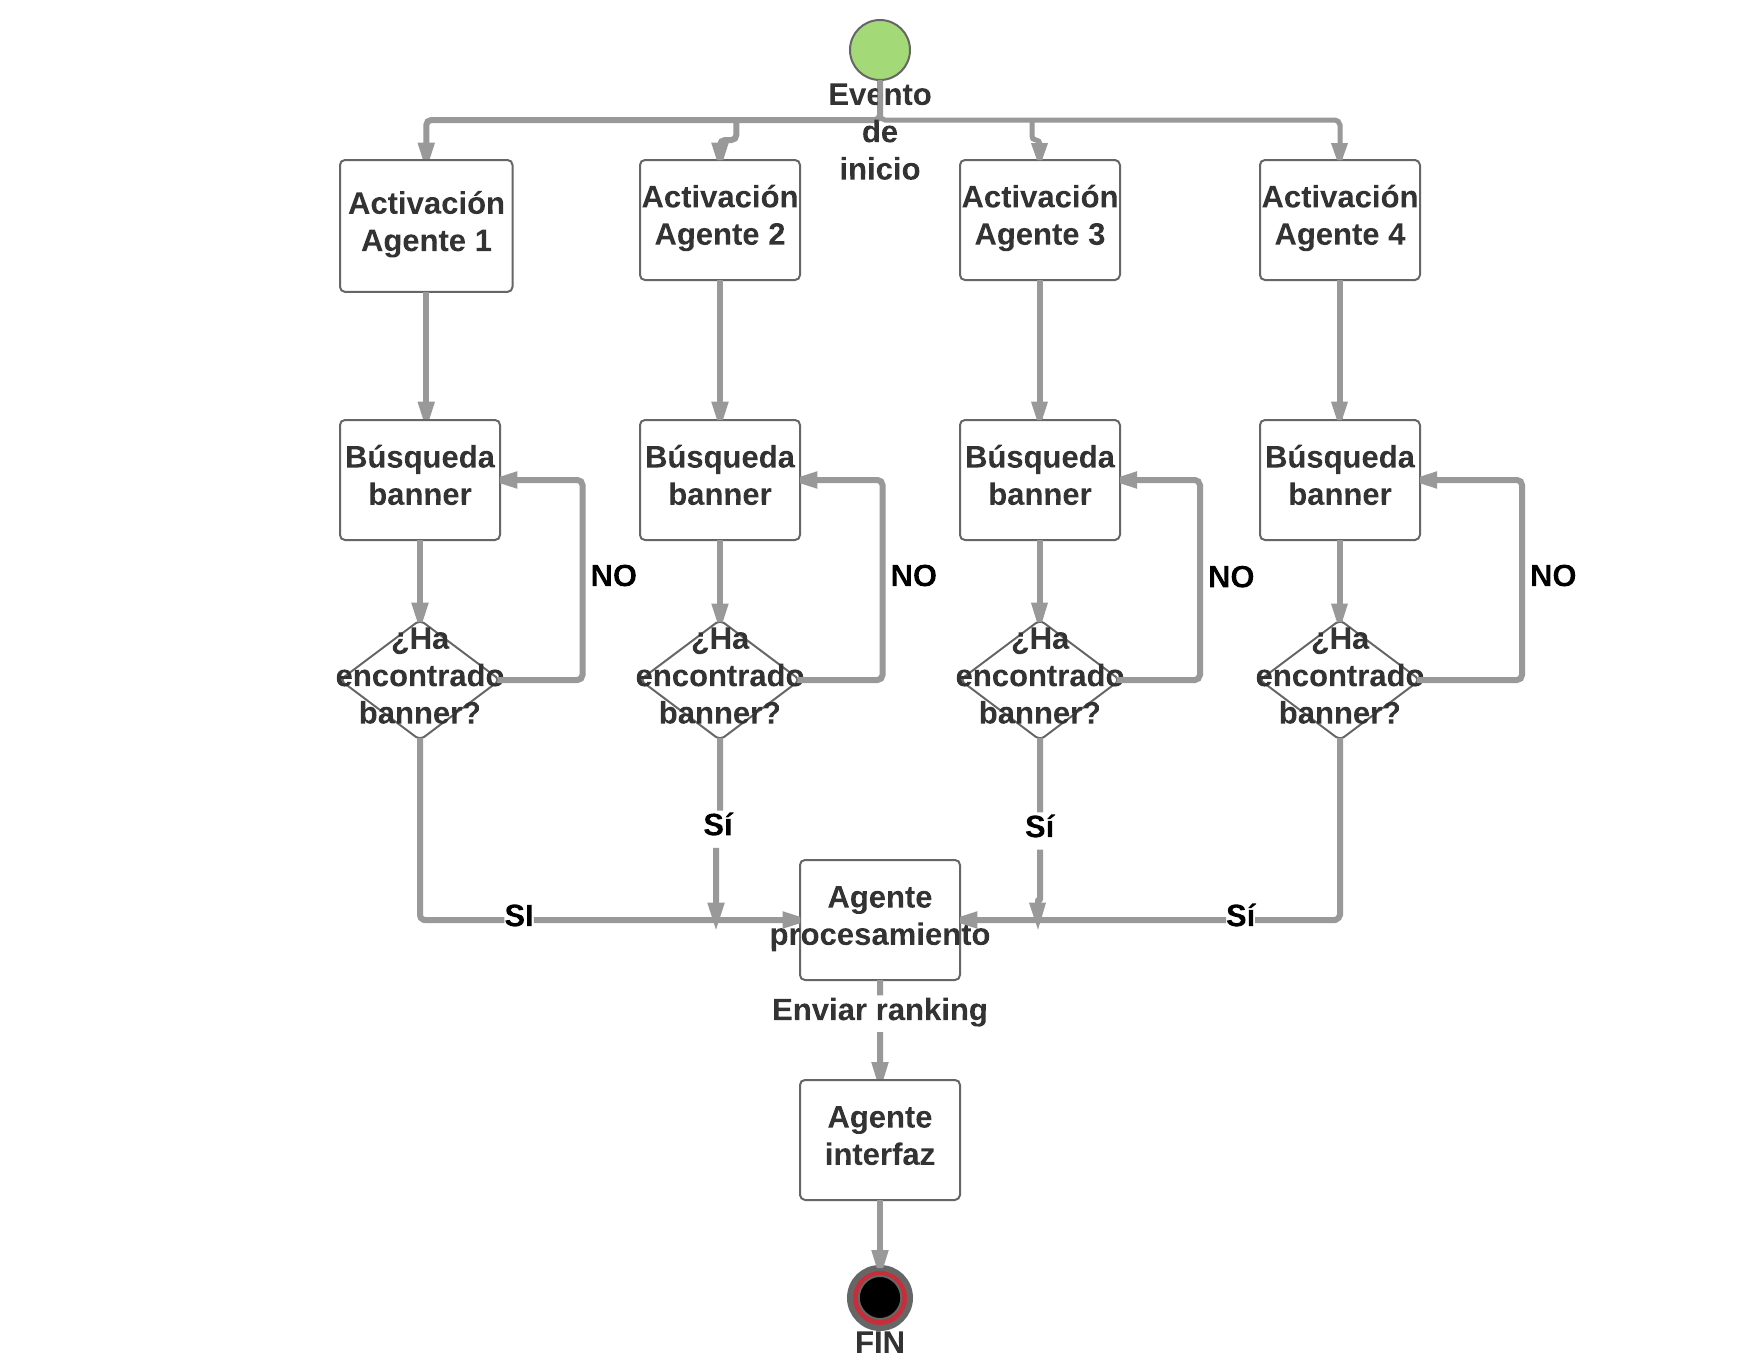
\includegraphics[width=1.0\textwidth]{flujo-sma}
    \caption{Diagrama de flujo del sistema multiagente}
    \label{fig:flujo-sma}
\end{figure}

\clearpage

\section{EJEMPLO}

Este ejemplo simula el comportamiento que tendría un agente de recuperación de links en una página cualquiera.

\begin{lstlisting}[caption=Ejemplo de código de recuperación de links de una URL,style=java]

/**
 * Example program to list links from URL. 
 */
package sample;

import org.jsoup.Jsoup;
import org.jsoup.nodes.Document;
import org.jsoup.nodes.Element;
import org.jsoup.select.Elements;

import java.io.IOException;

/**
 * @author Alberto Aranda Garcia y Cristian Gomez Portes
 */
public class ListLinks {
    public static void main(String[] args) throws IOException {
        String url = "http://www.marca.com/"; // Test URL
        print("Fetching %s...", url);

        Document doc = Jsoup.connect(url).get();
        Elements links = doc.select("a[href]");
        Elements media = doc.select("[src]");

        print("\nMedia: (%d)", media.size());
        for (Element src : media) {
            if (src.tagName().equals("img"))
                print(" * %s: <%s> %sx%s (%s)",
                        src.tagName(), src.attr("abs:src"), src.attr("width"), src.attr("height"),
                        trim(src.attr("alt"), 20));
            else
                print(" * %s: <%s>", src.tagName(), src.attr("abs:src"));
        }

        print("\nLinks: (%d)", links.size());
        for (Element link : links) {
            print(" * a: <%s>  (%s)", link.attr("abs:href"), trim(link.text(), 35));
        }
    }

    private static void print(String msg, Object... args) {
        System.out.println(String.format(msg, args));
    }

    private static String trim(String s, int width) {
        if (s.length() > width)
            return s.substring(0, width-1) + ".";
        else
            return s;
    }
}

\end{lstlisting}

En el siguiente enlace se muestra el contenido del archivo ``blacklist'': \url{https://github.com/aarandag/ClassifiAds/blob/master/blacklist.txt}.

\newpage

\bibliographystyle{alpha}
\singlespacing
\bibliography{ejemplo}


\end{document}


% Local Variables:
% coding: utf-8
% mode: flyspell
% ispell-local-dictionary: "castellano8"
% mode: latex
% End:
